\chapter{Theoretische Grundlagen}
Die Entwicklung einer neuen Messtechnik für das Fahrrad und den Flying Suit stellt eine komplexe Aufgabe da.
Dies beinhaltet die Planung und Bestellung nötiger Materialien und die Anbringung dieser am jeweiligen Aufbau.
Um sicherzustellen, dass die zu entwickelnde technische Umsetzung möglich ist, wurde das Zusammenspiel von Node und Dehnungsmessstreifen zunächst am einfacheren Aufbau eines Biegebalkens getestet.



\section{Drahtlose Sensornetzwerke und der V-Link 200 \(Menzel\)}

Dies soll durch die Verwendung des VLINK200 Nodes der Herstellers LORD/HBK stattfinden.
Dieses Unternehmen bietet Lösungen für drahtlose Sensornetzwerke an. Diese werden in der Industrie und dem Internet of Things, sowie auch in der Forschung und im Maschinen und Anlagenbau verwendet.
Dort wird sie vor allem im Bereich der predictive Maintenance eingesetzt.
Der Node verfügt über 8 Eingänge, 4 ±156mV Differenzeingänge und 4 ± 156mV Single-Ended Eingänge.
Er gewährleistet eine verlustfreie Datenübertragung sowie auch die Speicherung von Messdaten.
Man kann den Node über interne, austauschbare Batterien und externe Akkus betreiben.

\begin{figure}[h]
    \begin{center}
        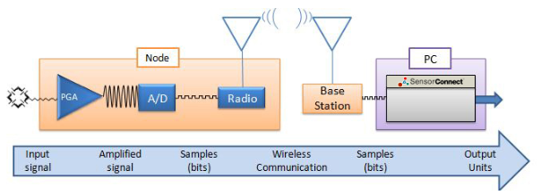
\includegraphics[width=1\textwidth, keepaspectratio]{lord_wireless.png}
        \caption[LORD drahtlose Übertragung (Abbildungsverzeichnis)]{LORD drahtlose Übertragung
        \cite{VLInkManual}
        }
        \label{fig:lordwireless}
    \end{center}
\end{figure}

Abbildung \ref{fig:lordwireless} zeigt die Funktionsweise der drahtlosen Datenübertragung.
Ein an das Node angeschlossener Sensor wird inerhalb des Nodes verstärkt und digitalisiert.
Anschließend werden die Messdaten vom Node drahtlos an eine Base Station gesendet welche mit einem Laptop verbunden ist.
Dort kann durch die Software SensorConnect auf den Node zugegriffen werden und dessen Daten visualisiert oder weiter verarbeitet werden.


Abbildung \ref{fig:lordproducts} zeigt einen Teil der Produktpalette.
Als Gateway wurde von uns der dort gezeigte USB Stick genutzt.
Insgesamt wurden uns zwei VLINK 200 Node, und ein USB Stick zur Verfügung gestellt was in der späten Projektphase teilweise zu Problemen führte,
siehe \ref{sec:probleme} \nameref{sec:probleme}.

\begin{figure}[h]
    \begin{center}
        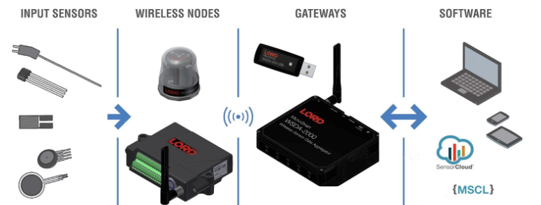
\includegraphics[width=1\textwidth, keepaspectratio]{lord_products.png}
        \caption[LORD Produkte (Abbildungsverzeichnis)]{LORD Produkte
        \cite{VLInkManual}
        }
        \label{fig:lordproducts}
    \end{center}
\end{figure}

\section{Dehnungsmessstreifen und Messprinzipien \(Bellgardt\)}




\section{Biegebalken \(Menzel\)}
\subsection{Aufbau des Biegebalkens}
Auf der Ober- und Unterseite des Biegebalkens sind Dehnungsmessstreifen angebracht um die beim aufbringen eines Gewichts entstehende Dehnung messen zu können.
Dies wurde mit verschiedenen Gewichten und in verschiedenen Einheiten durchgeführt.
\begin{figure}[h]
    \begin{center}
        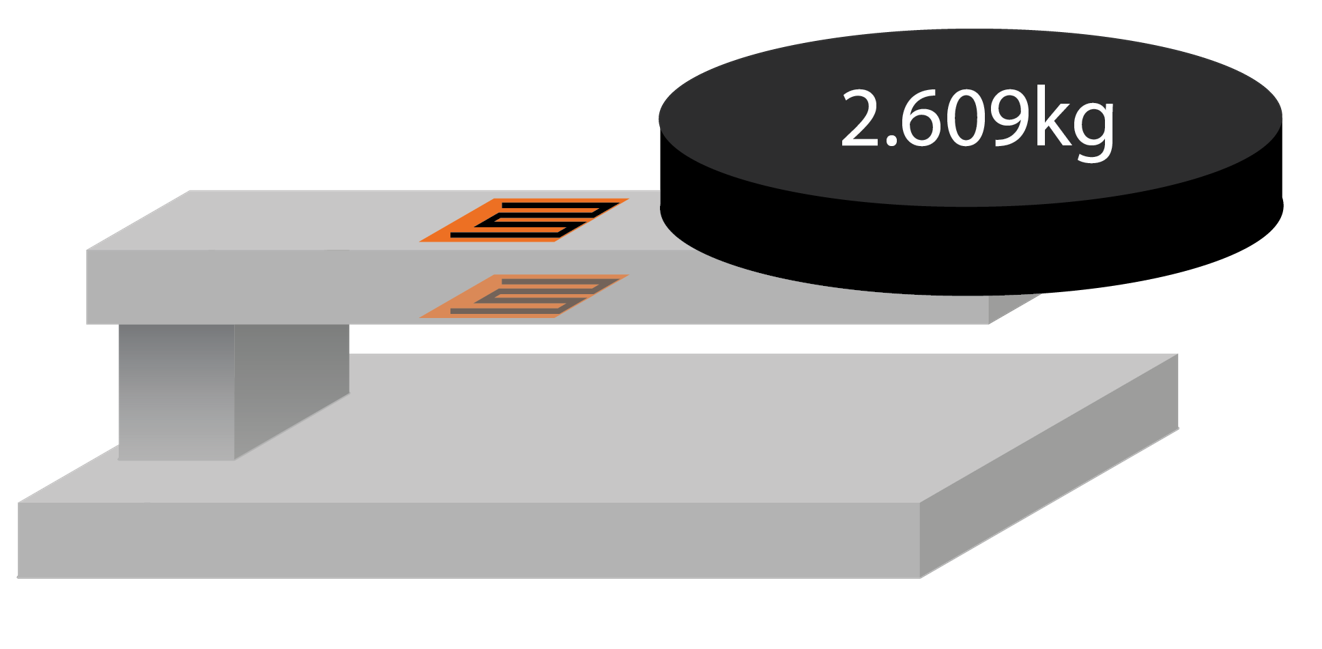
\includegraphics[width=0.5\textwidth, keepaspectratio]{biegebalken_grafik.png}
        \caption[Biegebalken Schema (Abbildungsverzeichnis)]{Biegebalken Schema
        %\cite{VLInkManual}
        }
        \label{fig:biegebalkenschema}
    \end{center}
\end{figure}

\subsection{Wahl des Messverfahrens}
Um Messungen durchführen zu können bieten sich verschiedene Verfahren an.
Die in der Software SensorConnect verfügbaren und für uns relevanten Verfahren sind die Shunt-, Field-, und Sensitivity(geometriebasierte)-kalibrierung.
Die Beschreibung sowie die Vor- und Nachteile dieser Verfahren sind in \ref{tbl:verfahren} \nameref{tbl:verfahren} dargestellt.
Um die theoretische Grundlage für den Aufbau des Fahrrads und des Flying Suits zu schaffen wurde sich beim Biegebalken für die Wahl des mV/V Messverfahrens entschieden.

\bgroup
\def\arraystretch{2}
\begin{table}[h]
\centering
\begin{tabular}{|p{0.25\linewidth}|p{0.25\linewidth}|p{0.25\linewidth}|p{0.25\linewidth}|}
\hline
Verfahren & Beschreibung & Vorteil & Nachteil\\ \hline
Shunt Kalibrierung & Interner (Shunt) Widerstand wird zur DMS-Brücke geschaltet. Es wird eine definierte Dehnung simuliert, um die Messkette zu überprüfen.
& schnell, einfach & Simuliert keine echte mech. Belastung, nur elektrische Effekte
\\ \hline
Field Kalibrierung & Messung von realer mech. Belastung mit Referenzlast

& Wenn Last bekannt ist, kann man sehr genau messen.
& Definierte Belastung der Struktur notwendig

\\ \hline
Geometriebasierte Kalibrierung (mV/V)
 & Berechnung für Software basierend auf Materialparametern und Geometrie


& Ermöglicht eine Abschätzung und Vergleich zwischen erwarteten und gemessenen Werten

& Abweichungen bei ungenauen Materialparametern möglich


\\ \hline

\end{tabular}
\caption{Messverfahren}
\label{tbl:verfahren}

\end{table}
\egroup


\subsection{Berechnung der Sensitivity}
Um eine Messung am Biegebalken durchführen zu können wurde zunächst die Sensitivity mathematisch berechnet.
Sie basierst auf der Geometrie des Biegebalkens, sowie des zu erwartendem maximalen Gewicht und wird als Parameter in SensorConnect eingegeben.
Sie stellt den gemessenen Wert in mV/V bei Maximalbelastung dar.
Aufgrund der einfachen Geometrie des Biegebalkens ist dies ein wichtiger Schritt, bevor diese für die komplexere Geometrie des Fahrradlenkers oder des Gestells des Flying Suits berechnet wird.

In der folgenden Berechnung wird für den Parameter n der Wert 2 verwendet, da es sich um die Anzahl der angebrachten DMS und die daraus resultierende Brückenkonfiguration handelt.
Der Parameter k ist durch die verwendeten DMS gegeben. Als maximale Last dient eine Hantelscheibe mit einem Gewicht von 2.609kg.



Maße des Biegebalkens:
\[
l = 117 \text{ mm}, \quad b = 19.8 \text{ mm}, \quad h = 2.94 \text{ mm}
\]
Maximale Last:
\[
M = 2.609 \text{ kg}
\]

\subsection*{Berechnung des Widerstandsmoments}
\[
W_x = \frac{b h^2}{6}
\]
Einsetzen der Werte:
\[
W_x = \frac{19.8 \times 2.94^2}{6} = 28.52 \text{ mm}^3
\]

\subsection*{Berechnung des Biegemoments}
\[
M_b = F \times l
\]
\[
M_b = 2.609 \times 9.81 \times 117mm = 2994.53 \text{ Nmm}
\]

\subsection*{Berechnung der Spannung}
\[
\sigma = \frac{M_b}{W_x}
\]
\[
\sigma = \frac{2994.53}{28.52} = 104.99 \text{ N/mm}^2
\]

\subsection*{Berechnung der Dehnung}
\[
\varepsilon = \frac{\sigma}{E}
\]
Mit \(E = 210000 \text{ N/mm}^2\):
\[
\varepsilon = \frac{104.99}{210000} = 0.499\times 10^{-3}
\]

\subsection*{Berechnung der Brückenausgabe}
\[
\frac{U_M}{U_B} = \frac{n}{4} \times k \times \varepsilon
\]
Mit \( n = 2 \), \( k = 2.01 \):
\[
\frac{U_M}{U_B} = \frac{2}{4} \times 2.01 \times 0.499 \times 10^{-3}
\]
\[
\frac{U_M}{U_B} = 0.000502 \text{ V/V} = 0.5 \text{ mV/V}
\]

Mit der berechneten Sensitivity wurden mehrere Messungen durchgeführt.
Die erste Messung wurde mit einem Gewicht von 2.609kg durchgeführt und in MPa gemessen, siehe \ref{tbl:biegebalkenmessungeins} \nameref{tbl:biegebalkenmessungeins}.

\bgroup
\def\arraystretch{2}
\begin{table}[h]
\centering
\begin{tabular}{|p{0.33\linewidth}|p{0.33\linewidth}|p{0.33\linewidth}|}
\hline
Gegeben & Gemessen & Abweichung \\ \hline
105MPa (2.609kg) & 120MPa (2.8kg) & +14\% \\ \hline
\end{tabular}
\caption{Messung 1 mit Maximalgewicht, [MPa]}
\label{tbl:biegebalkenmessungeins}

\end{table}
\egroup

Die zweite Messung wurde mit verschiedenen Gewichten getestet und in N gemessen, siehe \ref{tbl:biegebalkenmessungzwei} \nameref{tbl:biegebalkenmessungzwei}.
\bgroup
\def\arraystretch{2}
\begin{table}[h]
\centering
\begin{tabular}{|p{0.33\linewidth}|p{0.33\linewidth}|p{0.33\linewidth}|}
\hline
Gegeben & Gemessen & Abweichung \\ \hline
0N (0kg) & 0.2N (0.02kg) & - \\ \hline
3.9N (0.4kg) & 4.6N (0.46kg) & +17.9\%  \\ \hline
24.5N (2.609kg) & 27.6N (2.81kg)  & +12.6\% \\ \hline
\end{tabular}
\caption{Messung 2, [N]}
\label{tbl:biegebalkenmessungzwei}

\end{table}
\egroup


\section{Viertel\-, Halb\- und Vollbr\"uckenschaltungen für DMS \(Bellgardt\)}
\section{Mechanische Belastungen (Biegung, Torsion, Kr\"afte) \(Bellgardt, Menzel\)}